\documentclass{standalone}
\usepackage{tikz}
\usepackage{verbatim}
\usetikzlibrary{positioning}
\begin{document}
\pagestyle{empty}
  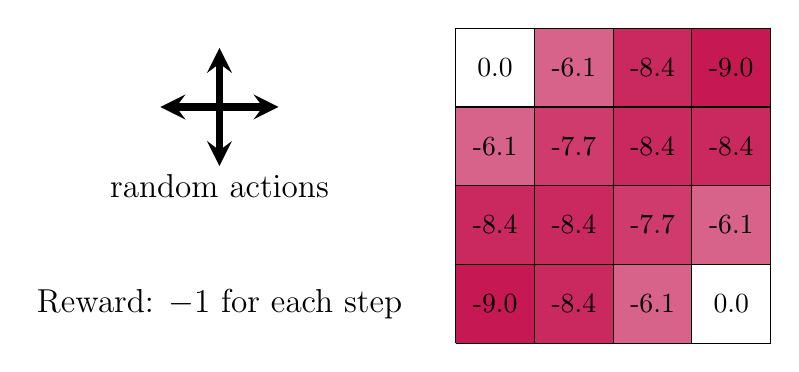
\begin{tikzpicture}
    \draw[stealth-stealth, line width=1 mm] (-3.75, 3) -- (-2.25, 3);
    \draw[stealth-stealth, line width=1 mm] (-3, 2.25) -- (-3, 3.75);
    \node at (-3, 2) {\large random actions};
    \node at (-3, 0.5) {\large Reward: $-1$ for each step};
    % Top row.
    \node at (0.5, 3.5) {0.0};
    \fill[purple!61] (1, 3) rectangle (2,4);
    \node at (1.5, 3.5) {-6.1};
    \fill[purple!84] (2, 3) rectangle (3,4);
    \node at (2.5, 3.5) {-8.4};
    \fill[purple!90] (3, 3) rectangle (4,4);
    \node at (3.5, 3.5) {-9.0};
    % Second frop top row.
    \fill[purple!61] (0, 2) rectangle (1,3);
    \node at (0.5, 2.5) {-6.1};
    \fill[purple!77] (1, 2) rectangle (2,3);
    \node at (1.5, 2.5) {-7.7};
    \fill[purple!84] (2, 2) rectangle (3,3);
    \node at (2.5, 2.5) {-8.4};
    \fill[purple!84] (3, 2) rectangle (4,3);
    \node at (3.5, 2.5) {-8.4};
    % Second from bottom row.
    \fill[purple!84] (0, 1) rectangle (1,2);
    \node at (0.5, 1.5) {-8.4};
    \fill[purple!84] (1, 1) rectangle (2,2);
    \node at (1.5, 1.5) {-8.4};
    \fill[purple!77] (2, 1) rectangle (3,2);
    \node at (2.5, 1.5) {-7.7};
    \fill[purple!61] (3, 1) rectangle (4,2);
    \node at (3.5, 1.5) {-6.1};
    % Bottom row.
    \fill[purple!90] (0, 0) rectangle (1,1);
    \node at (0.5, 0.5) {-9.0};
    \fill[purple!84] (1, 0) rectangle (2,1);
    \node at (1.5, 0.5) {-8.4};
    \fill[purple!61] (2, 0) rectangle (3,1);
    \node at (2.5, 0.5) {-6.1};
    \node at (3.5, 0.5) {0.0};
    \draw[step=1.0,black] (0,0) grid (4, 4);
  \end{tikzpicture}
\end{document}